\documentclass[11pt]{article}

\usepackage[
  paperwidth=8.5in,
  paperheight=36in,
  left=0.8in,
  right=0.8in,
  top=0.8in,
  bottom=1.5in,
]{geometry}
\usepackage{amsmath,amssymb}
\usepackage{graphicx}

\usepackage{tikz}
\usetikzlibrary{arrows.meta, positioning, fit, backgrounds, calc}


\usepackage[dvipsnames]{xcolor}
\usepackage{hyperref}
\definecolor{okabepink}{HTML}{CC79A7}
\definecolor{okabecyan}{HTML}{56B4E9}
\hypersetup{
  colorlinks = true,
  linkcolor  = black,
  citecolor  = black,
  urlcolor   = okabepink
}

\usepackage{listings}
\usepackage[most]{tcolorbox}
\tcbuselibrary{listings}

\definecolor{codebg}{RGB}{248,248,248}
\definecolor{codeframe}{RGB}{225,225,225}
\definecolor{codekw}{RGB}{120,70,160}
\definecolor{codecomment}{RGB}{100,120,100}
\definecolor{codestring}{RGB}{160,80,60}
\definecolor{codeattr}{RGB}{80,100,150}

\lstdefinelanguage{Rust}{
  sensitive=true,
  keywords={
    as,break,const,continue,crate,else,enum,extern,false,fn,for,if,impl,in,
    let,loop,match,mod,move,mut,pub,ref,return,self,Self,static,struct,
    super,trait,true,type,unsafe,use,where,while,async,await,dyn
  },
  keywordstyle=\color{codekw}\bfseries,
  comment=[l]{//},
  morecomment=[s]{/*}{*/},
  commentstyle=\color{codecomment}\itshape,
  morestring=[b]",
  stringstyle=\color{codestring},
  alsoletter={\#},
  moredelim=[s][\color{codeattr}]{\#[}{]},
}

\newtcblisting{rust}{
  listing engine=listings,
  listing only,
  colback=codebg,
  colframe=codeframe,
  boxrule=0.35pt,
  arc=2pt,
  left=10pt,
  right=10pt,
  top=9pt,
  bottom=9pt,
  width=\textwidth,
  before skip=0.8em,
  after skip=0.9em,
  listing options={
    language=Rust,
    basicstyle=\ttfamily\small,
    breaklines=true,
    columns=fullflexible,
    keepspaces=true,
    showstringspaces=false,
    tabsize=4,
    upquote=true
  }
}
\usepackage{enumitem}
\newlist{notelist}{itemize}{1}
\setlist[notelist]{
    label={--},
    leftmargin=2.0em,
    itemsep=0.2em,
    topsep=0.4em,
    parsep=0em
}

\title{
  Safe Interface Design for a Minimal BLAS-like Kernel Library \\[0.25em]
  \large LAK Working Note \#1
}
\author{
  deval-d@stanford.edu 
}

\date{08 May 2026}

\begin{document}

\maketitle
\thispagestyle{empty} 

\begin{abstract}
\texttt{lak} is a small BLAS-like kernel library being written in safe Rust. Its goal is not to reproduce the full BLAS interface, but to explore how clean a contiguous-memory API can get when you are not bound by historical constraints. The guiding question is whether a safe, idiomatic Rust interface can stay minimal and elegant, sacrificing nothing in the level-1 and level-2 BLAS, and nothing serious in the level-3 BLAS.
\end{abstract}

\section{LAK}

Basic Linear Algebra Subprograms (\href{https://www.netlib.org/blas/}{BLAS})
is a standardized set of routines for common linear algebra operations: vector
addition, scalar multiplication, dot products, matrix-vector products, and
matrix multiplication. These routines are the most important building blocks in numerical computing.
Libraries like \href{https://github.com/flame/blis}{BLIS}, Intel's \href{https://www.intel.com/content/www/us/en/developer/tools/oneapi/onemkl.html}{MKL},
Apple \href{https://developer.apple.com/documentation/accelerate}{Accelerate},
and \href{https://github.com/OpenMathLib/OpenBLAS}{OpenBLAS} have been refined
over years to make these small primitives run as efficiently as possible across
many different architectures.

\texttt{linalg-kernels}, or \texttt{lak}, is a small BLAS-like linear algebra
library being written in safe Rust. It is not meant to be a BLAS implementation. Other mature Rust libraries for fast numerical linear algebra, such as
\href{https://faer.veganb.tw}{\texttt{faer}} or
\href{https://nalgebra.rs}{\texttt{nalgebra}} also already exist. I am writing \texttt{lak}
mainly to learn how these routines are designed and written to be fast.
There is also a design question behind the project. If I do not try to support
the entire historical interface, and instead focus on contiguous memory,
simple views, and safe Rust wrappers, how clean can the code be while still
matching perf for unit-stride BLAS? These working notes are my attempt to explain
that process as I learn it.


\section{Safe Interface Design}

The standard BLAS interface operates on descriptors:
\begin{notelist}
    \item vectors: \;\;\((x_{\mathrm{ptr}}, \,n, \,\mathrm{incx})\)
    \item matrices: \((A_{\mathrm{ptr}}, \,m, \,n, \,\mathrm{lda})\)
    \item scalars: \;\;\:\((\alpha, \,\beta)\)
\end{notelist}
It assumes the caller has provided consistent sizes, strides, and leading
dimensions: \(n\), \(\mathrm{incx}\), and \(\mathrm{lda}\). The caller is
therefore responsible for matching shapes to descriptors, avoiding invalid aliasing between mutable arguments, and
distinguishing read-only inputs from mutable outputs.
If any of these assumptions are wrong, the failure mode is not usually a helpful
error. It is undefined behavior (UB): out-of-bounds reads, out-of-bounds writes, or
silent memory corruption. The tradeoff is that BLAS routines can expose a very small FFI-friendly low-level interface
and let implementations operate directly on raw pointers, without carrying
high-level shape information or performing bounds checks inside the inner
kernels that make the routine fast. Because  numerical linear algebra is everywhere, this tradeoff
is fine. BLAS-based libraries make UB a 
non-issue for most users. Even so, this design is anti-Rust. I sacrifice
the portability of the standard BLAS interface in exchange for one that is
idiomatic Rust, and only in Rust. 

\subsection{Vectors and Matrices}

\texttt{lak} only works with contiguous memory, so BLAS $\mathrm{incx}$ strides are unnecessary
and $n$ can be inferred directly from the length of the vector's buffer. Only a buffer is needed.

\begin{rust}
/// immutable vector type 
#[derive(Clone, Copy, Debug)]
pub struct VecRef<'a, T> { 
    buffer: &'a [T], 
}

/// mutable vector type
#[derive(Debug)]
pub struct VecMut<'a, T> { 
    buffer: &'a mut [T], 
}
\end{rust}
The \texttt{Ref}/\texttt{Mut} split makes read-only and mutable roles explicit. Matrices are similar,
though $(m, n)$ dimensions must be supplied explicitly, since the buffer alone does not encode the logical shape.

\begin{rust}
/// immutable matrix type 
/// stored in column-major order
#[derive(Clone, Copy, Debug)]
pub struct MatRef<'a, T> { 
    buffer: &'a [T], 
    dimension: (usize, usize), 
}

/// mutable matrix type 
/// stored in column-major order
#[derive(Debug)]
pub struct MatMut<'a, T> { 
    buffer: &'a mut [T],
    dimension: (usize, usize), 
}
\end{rust} 
The \verb|Mat|\footnote{\href{https://faer.veganb.tw}{\texttt{faer}} has the same matrix naming convention.} constructors validate that the dimension and buffer are mutually consistent.
The connecting thread across both types is that shape information lives in the wrapper,
not in the caller's head. Every kernel is now allowed to assume:
\begin{notelist}
    \item vector lengths are known from the slice length;
    \item matrix dimensions are checked when the view is constructed;
    \item immutable inputs and mutable outputs are separated by the type system;
    \item mutable aliases cannot be created through the safe interface;
    \item all storage is contiguous and column-major.
\end{notelist}
Invalid descriptors are ruled out before routines are called and inner kernels can remain safe: \\[1em]

\begin{figure}[h]
\centering
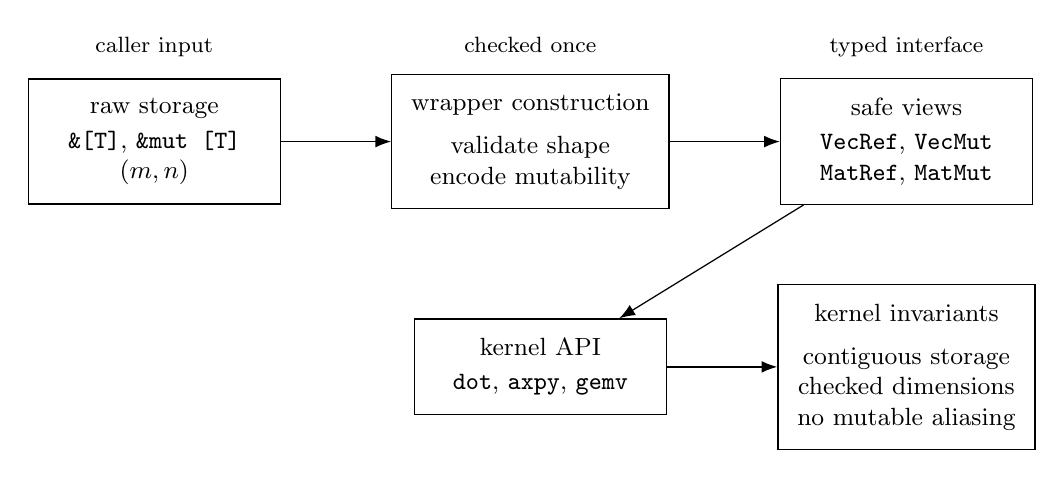
\begin{tikzpicture}[
    font=\small,
    node distance=1.25cm,
    box/.style={
        draw=black,
        fill=white,
        rectangle,
        minimum height=1.0cm,
        align=center,
        inner sep=7pt,
        line width=0.45pt
    },
    stage/.style={
        box,
        minimum width=3.2cm
    },
    invariant/.style={
        box,
        minimum width=3.7cm
    },
    arrow/.style={
        -{Latex[length=2mm]},
        line width=0.45pt,
        draw=black
    },
    label/.style={
        font=\footnotesize,
        text=black,
        align=center
    }
]

\node[stage] (raw) {
    raw storage\\[0.15em]
    \verb|&[T]|, \verb|&mut [T]|\\
    \((m,n)\)
};

\node[stage, right=1.4cm of raw] (wrap) {
    wrapper construction\\[0.5em]
    validate shape\\
    encode mutability
};

\node[stage, right=1.4cm of wrap] (safe) {
    safe views\\[0.15em]
    \texttt{VecRef}, \texttt{VecMut}\\
    \texttt{MatRef}, \texttt{MatMut}
};

\node[stage, below=1.0cm of safe] (inv) {
    kernel invariants\\[0.5em]
    contiguous storage\\
    checked dimensions\\
    no mutable aliasing
};

\node[stage, left=1.4cm of inv] (kernel) {
    kernel API\\[0.15em]
    \texttt{dot}, \texttt{axpy}, \texttt{gemv}
};

\draw[arrow] (raw) -- (wrap);
\draw[arrow] (wrap) -- (safe);
\draw[arrow] (safe) -- (kernel);
\draw[arrow] (kernel) -- (inv);

\node[label, above=0.15cm of raw] {caller input};
\node[label, above=0.15cm of wrap] {checked once};
\node[label, above=0.15cm of safe] {typed interface};

\end{tikzpicture}

\caption{The wrapper types move descriptor validity into construction. Once a
\texttt{VecRef}, \texttt{VecMut}, \texttt{MatRef}, or \texttt{MatMut} exists,
kernels can rely on contiguity, checked shape, and Rust's aliasing rules as
interface invariants.}
\label{fig:invariants}
\end{figure}

\subsection{Generic Kernels}

Restricting \texttt{lak} to Rust also naturally simplifies how routines are named and
implemented. The traditional BLAS interface has separate entry points for each
scalar type. For example, single-precision matrix-vector multiplication is
called through \texttt{sgemv}, while double-precision matrix-vector
multiplication is called through \texttt{dgemv}. This is natural for a C or
Fortran ABI, where the function name itself must encode the scalar type.
In \texttt{lak}, the public interface does not need separate routines for
\texttt{f32} and \texttt{f64}. A routine can be generic
over the scalar type:

\begin{rust}
pub fn gemv<T>(
    alpha: T, 
    beta: T, 
    a: MatRef<'_, T>, 
    x: VecRef<'_, T>, 
    y: VecMut<'_, T>
)
where
    T: Float,
    ...
{
    ...
}
\end{rust}

This removes a form of code duplication. Rust's 
monomorphization then produces machine code for each concrete
scalar type, so the generic interface does not introduce the overhead normally
associated with type erasure or dynamic dispatch. 

The difficulty is that different scalar types do not have the same performance
strategy. A double-precision value is twice as large as a single-precision value.
This changes how many elements fit in a cache line, how many elements fit in a SIMD
register, and how much matrix data fits in a fixed-size cache block (Figure \ref{fig:strategy}). For example, a cache block that holds \(N\) single-precision values only holds
\(N/2\) double-precision values. Similarly, a 128-bit SIMD register holds four
\texttt{f32} values but only two \texttt{f64} values. As a result, blocking
constants, unroll factors, and register-level kernels cannot always be shared
blindly between scalar types. A generic interface can expose one routine name,
but the implementation still has to respect the different storage and register
pressure of each type. One possible solution is to attach these constants to the scalar type itself.
However, Rust does not yet allow generic associated constants such as
\texttt{T::LANES} or \texttt{T::NC} to be used freely in const-generic
positions, and these constants may be different depending on the routine. SIMD widths and type-specific blocking constants thus remain implementation details.

For the level-1 and level-2 BLAS, this is easily manageable. 
These routines are limited more by memory traffic than by floating-point
throughput. The kernel spends much of its time streaming vectors or matrix
columns from memory, so the main requirement is to preserve simple contiguous
access and avoid unnecessary loads, stores, and bounds checks. The \textit{same}
constants tuned for \texttt{f64} can therefore often work well for \texttt{f32}.
The level-3 BLAS requires more care. Matrix multiplication has enough arithmetic
intensity that register blocking, cache blocking, packing layout, and SIMD width
become central to performance. 

\begin{figure}[h]
\centering
\begin{tikzpicture}[
    font=\small,
    matrix/.style={
        draw=black,
        fill=white,
        line width=0.5pt
    },
    f32block/.style={
        draw=black,
        fill=white,
        line width=0.5pt
    },
    f64block/.style={
        draw=black,
        fill=white,
        dashed,
        line width=0.5pt
    }
]


\draw[matrix] (0,0) rectangle (4,4);
\node[anchor=north east] at (3.75,3.75) {\Large \(A\)};

% f32 block: 2 x 2
\draw[f32block] (0,2) rectangle (2,4);
\node at (1.35,2.65) {\(\texttt{f32}\)};

% f64 block: 1 x 1
\draw[f64block] (0,3) rectangle (1,4);
\node at (0.5,3.5) {\(\texttt{f64}\)};

% ------------------------------------------------------------
% Right: footprint comparison
% ------------------------------------------------------------
\begin{scope}[xshift=7.0cm]
    \node at (1.45,4.45) {same byte span};
    % f32 footprint
    \draw[f32block] (0,0) rectangle (0.9,4);
    \node at (0.45,2) {\(\texttt{f32}\)};

    % f64 footprint, half height
    \draw[f64block] (2.0,2) rectangle (2.9,4);
    \node at (2.45,3) {\(\texttt{f64}\)};
\end{scope}

\end{tikzpicture}

\caption{The strategy depends on scalar width: double precision uses twice
as many bytes per value, so the same cache or SIMD span holds half as many
elements.}
\label{fig:strategy}
\end{figure}

\end{document}
